\chapter{Experiment}
This chapter begins by the experiment of simple three-branched wire harness for fast verification of key points detection methodology.
Followed by the experiment of wire harness with more branches to validate the feasibility in industry.
\section{Three branched wire harness}
In this section, the dataset used for training, generated model and the training's configuration and results will be introduced.
\subsection{Dataset}
The dataset consists of 100 images of three branched wire harnesses, see \autoref{fig:Three branched wire harness}. The dataset is split to 
two parts, 80 images for training and 20 images for validation.
In annotation,there are eight key points for each segment, which could be interpolated by cubic spline and formed as the wire spline model.
\begin{figure}[htbp]
    \centering
    \begin{subfigure}[b]{0.45\textwidth}
        \centering
        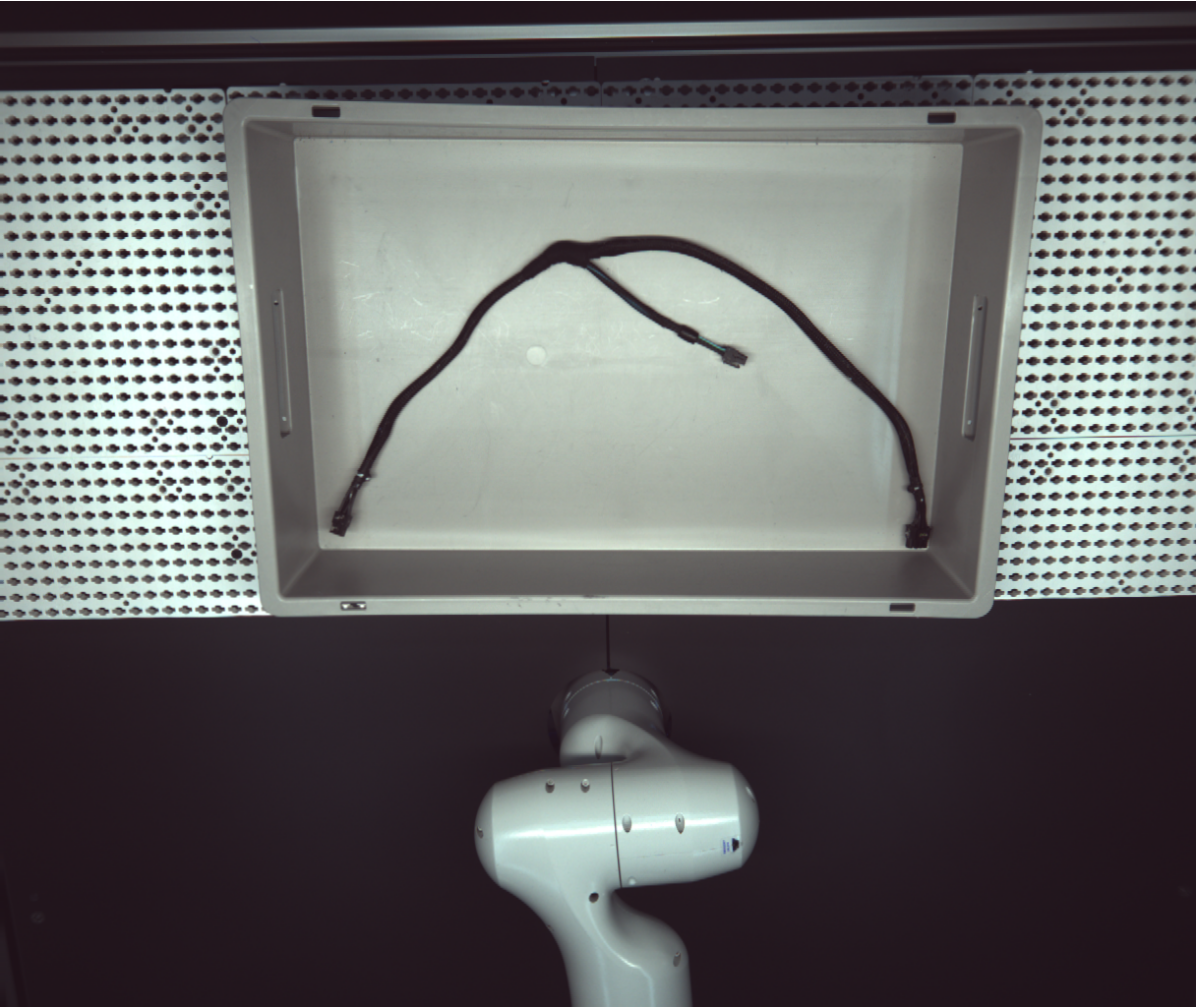
\includegraphics[width=0.9\linewidth]{example_images/img_0}
        \caption{Three branched wire harness without annotation}
        \label{fig:Three branched wire harness original}
    \end{subfigure}
    \hfill
    \begin{subfigure}[b]{0.45\textwidth}
        \centering
        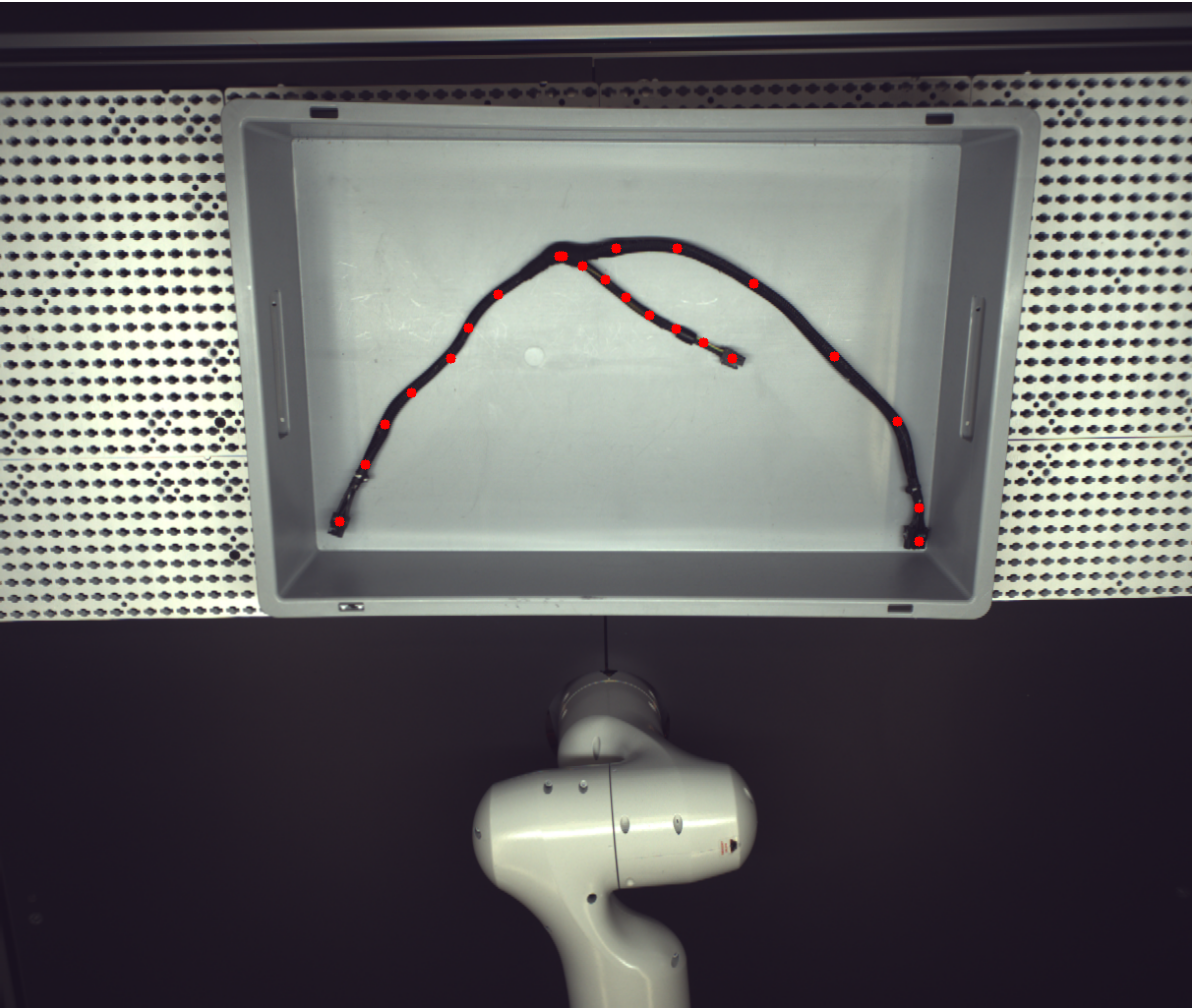
\includegraphics[width=0.9\linewidth]{example_images/img_0_anno}
        \caption{Three branched wire harness with annotation}
        \label{fig:Three branched wire harness with annotation}
    \end{subfigure}
    
    \caption{Three branched wire harness}
    \label{fig:Three branched wire harness}
\end{figure}
\subsection{Model}
The Model are composed of three parts: backbone, neck and head.\\
For this task, the Swin-Transformer is employed as backbone. After the backbone, features are extracted and the dimension of input image changes 
from 1x3x256x256 to 1x768x32x32. The image has a smaller size but deeper features.
Between them, there are also two stages and the feature dimensions are 192 and 384, respectively. 
The four stages will then be collected to feed into the neck, Feature Pyramid Networks. The output tensor of the FPN is upsampled in head by using
Transposed Convolution to reconstruct to task-specific dimensions.
In this case is 1x3x8x256x256, which means 3 segments, 8 key points and the image size is 256x256.
\subsection{Training} 
The model is trained with SGD optimizer and the batch size is 2. After 106 epochs, the loss will end with 1.28, see \autoref{fig:Training result}.\\
\begin{figure}
	\centering
	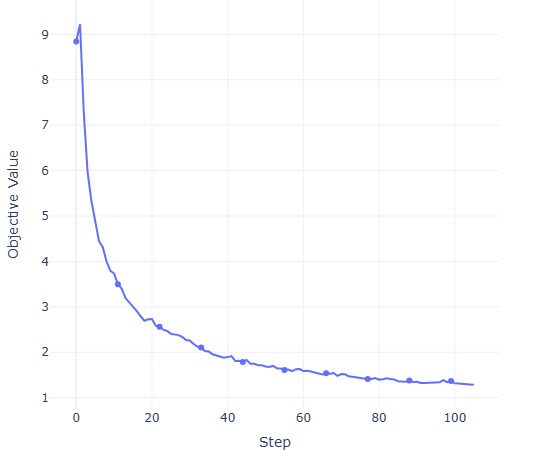
\includegraphics[width=0.6\linewidth]{example_images/noAttn_keypoints_100}
	\caption{Training results}
	\label{fig:Training result}
\end{figure}
The evaluated result is in \autoref{fig:Training result validation}. The result is not ideal, since several keypoints are incorrectly or
inaccurately detected, i.e., detected on the other segment, or outside the wire harnesses. The sequence of keypoints is also not correctly 
ordered, such that the interpolated spline looks not promising. Hence, the model should be optimized.
\begin{figure}
	\centering
	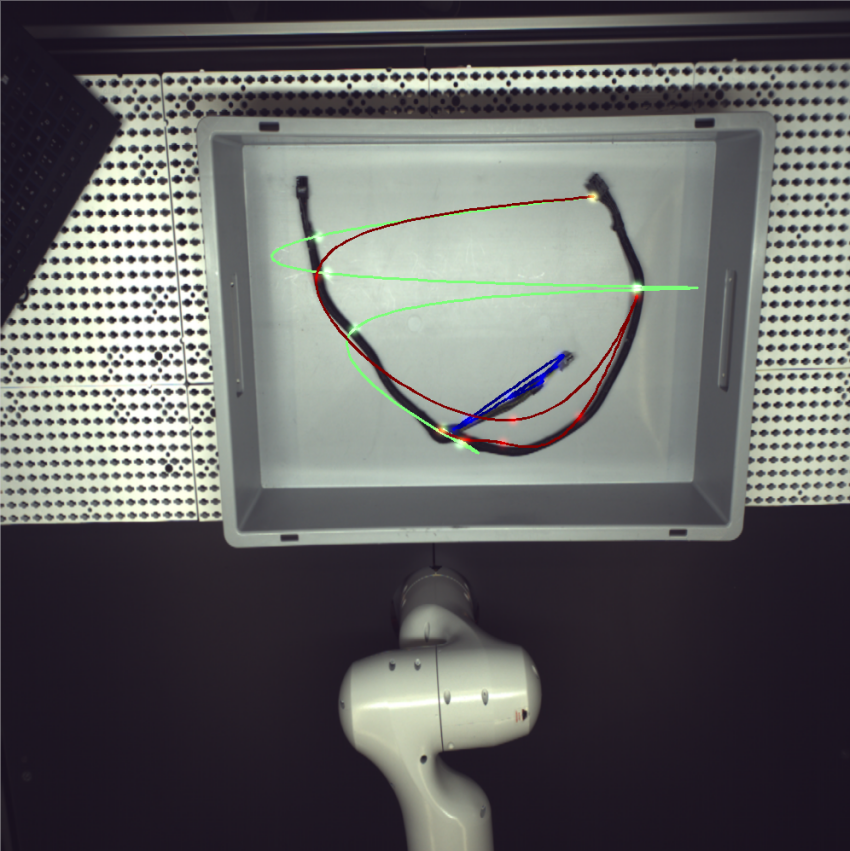
\includegraphics[width=0.6\linewidth]{example_images/noAttn_keypoints_100_eval}
	\caption{Validation}
	\label{fig:Training result validation}
\end{figure}
\subsection{Optimization}
\subsubsection{Self attention}
Since there are several keypoints are detected on the wrong segment. The attentional mechanism might could facilitate the model to pay attention 
to the highlights of the image so that the keypoints are correctly detected on the right segment. The encoder layers of transformer are placed in 
head during upsampling. After training the loss is decreased to 0.83 after 234 epochs, see \autoref{fig:Training result with Attention}. 
The evaluation is in \autoref{fig:Training result validation Attention}.\\
\begin{figure}
	\centering
	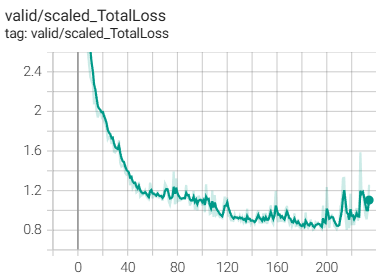
\includegraphics[width=0.6\linewidth]{example_images/withAttn_keypoints_100}
	\caption{Training result}
	\label{fig:Training result with Attention}
\end{figure}
\begin{figure}
	\centering
	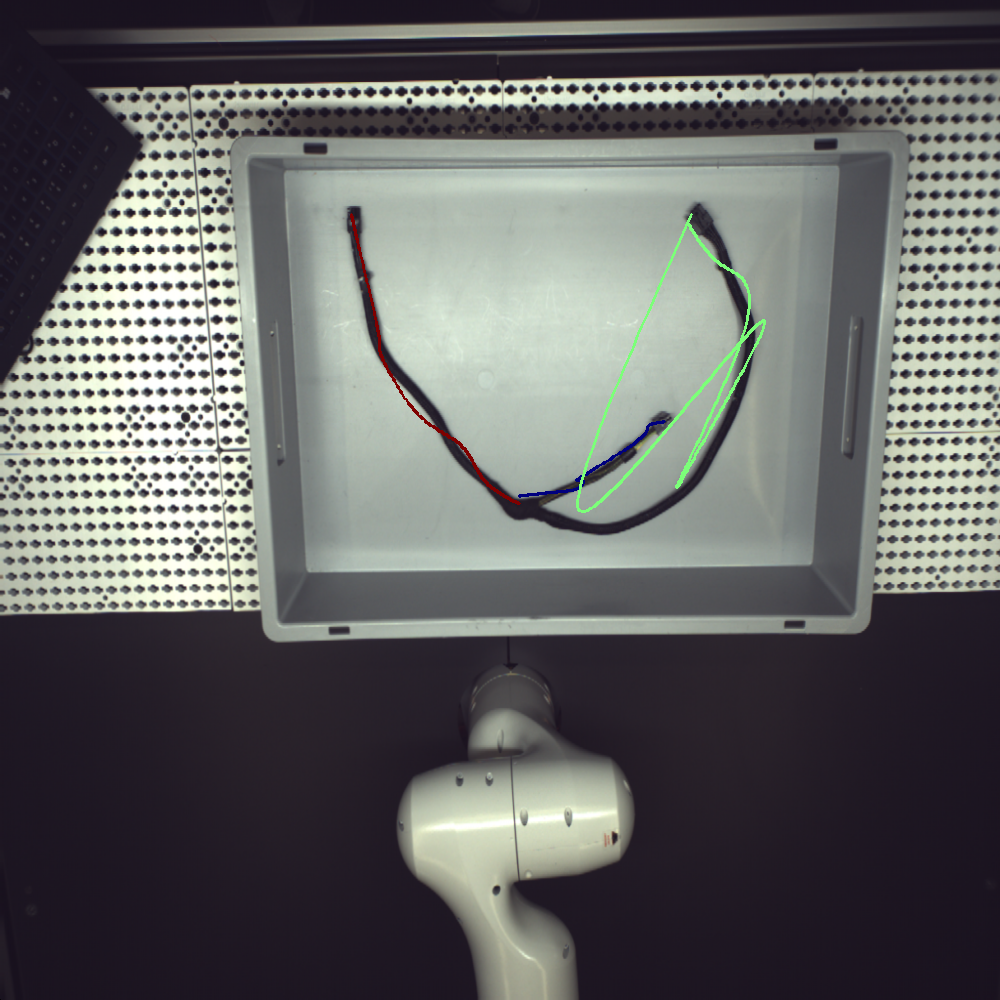
\includegraphics[width=0.6\linewidth]{example_images/keypoints_100_eval_withAttn}
	\caption{Validation for model with self attention}
	\label{fig:Training result validation Attention}
\end{figure}
The detection of keypoints is preciser than before. However, the sequence is still not correct.
To solve this problem, the keypoints are sorted before evaluation by using greedy algorithm. The keypoints are always gathered 
at the intersection at the beginning. Thus, the first point in the sequence of keypoints can be easily determined. After that the 
next point nearest to the first point will be found. Once this step has been done, the previous point is excluded from the list of 
following points to be searched. The point closest to the newly found point will continue to be found. This process is repeated 
until all the keypoints have been iterated. After the sort of keypoints, the result of evaluation is \autoref{fig:Training result validation Attention and Sort}.\\
\begin{figure}
	\centering
	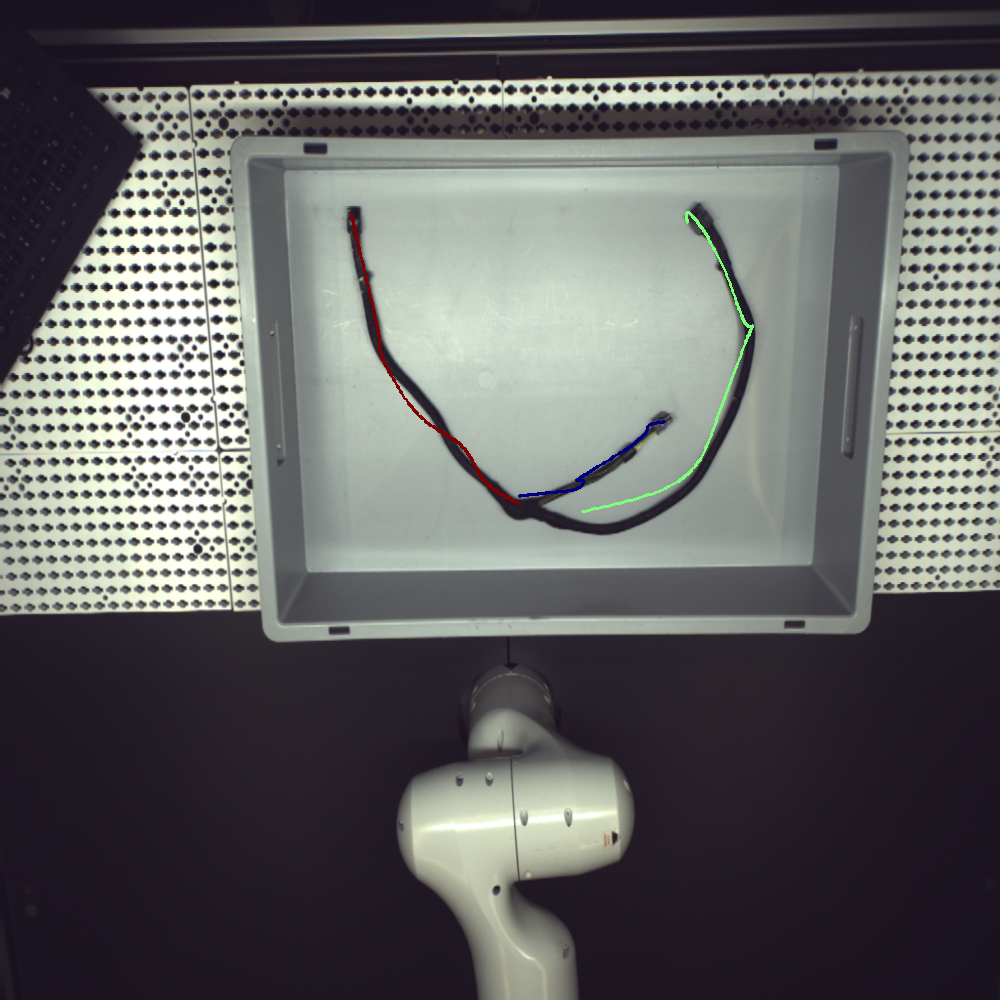
\includegraphics[width=0.6\linewidth]{example_images/withAttn_sort_keypoints_100_eval}
	\caption{Validation for model with sort of key points}
	\label{fig:Training result validation Attention and Sort}
\end{figure}
The keypoints are still at the same position, but the sequence of keypoints on each segment is sorted and the evaluation looks more reasonable. 
\subsection{Comparative experiment}
Several comparative experiments are done for evaluating the model.\\ 
\subsubsection{Resnet-50 as backbone}
Resnet-50 is used as the backbone to extract features in the first comparative experiment. The model is the nothing different but just the backbone is 
replaced. After the backbone, the dimension of the image changes from 1x3x256x256 to 1x2048x32x32. The validated loss will be decreased to 0.79 after 
177 epochs. The loss is $16\%$ higher than the model employed swin-transformer as backbone.  
\subsubsection{Resnet-50 as backbone}
Resnet-50 is used as the backbone to extract features in the first comparative experiment. The model is the nothing different but just the backbone is 
replaced. After the backbone, the dimension of the image changes from 1x3x256x256 to 1x2048x32x32. The validated loss will be decreased to 0.79 after 
177 epochs.
\subsubsection{YOLOV8}
YOLO V8 is a one stage object detection algorithm. The model after training could also predict the keypoints by using the coordinate regression method.
In contrast to the Heatmap method, the model predicts the coordinate of keypoints directly and compares it with the groundtruth. The dataset for YOLO is 
different from the dataset for the previous model. Each annotation file is in txt format and has one class "wire harness" and for each class there are eight 
keypoints, so after the training the model could also predict each segment individually. The model is still trained with the 100 images of wire harness.
The results are in \autoref{tab:Training results of YOLO}. The loss of validation is about 7 times higher than training loss and the model is over-fitting.
The generalization of the model is worse than the previous. \\
\begin{table}[htb]
    \centering
    \begin{tabular}{@{}llr@{}} \toprule
    \multicolumn{2}{c}{Result}             \\ \cmidrule(r){1-2}
                 & Loss   \\ \midrule
        Training & 0.9    \\
        Validation& 6.5    \\ \bottomrule
    \end{tabular}
    \caption{Training results of YOLO} 
    \label{tab:Training results of YOLO}
    \end{table}
In order to test the coordinate regression method further, inspired by YOLO, the head of the previous model was modified to use the coordinate regression method.
The Dataset is the same and after the training, the validation loss is double of the previous validation loss. At least for small dataset, the coordinate regression
method is not suitable.
\subsection{Dataset expansion}
Using a small dataset like previous is good for fast verifying the idea. However, a dataset that is too small may lead to: 
\begin{itemize}
	\item Overfitting
	\item High Variance of the model parameters
	\item Difficult in evaluation
	\item Inaccurate model predictions
\end{itemize}
Therefore, it is essential to find ways to expand the dataset. In this subsection, we experiment with two methods for expanding the dataset. They are:
1) Wire bundle images generated by CycleGAN. 2) Composition of new wire harness images by rotating, translating on the branches of the original image. 
The models are pre-trained using the two methods, respectively. After obtaining satisfactory results, the model is subjected to transfer learning using 
the previous dataset to explore whether the pre-training has improved the predictive ability of the model.
\subsubsection{Expand Dataset by CycleGAN}
Generating the virtual images of the wire harness using the CycleGAN network requires first generating images of the simple three-branched-spline curve 
obtained by sketching \autopageref{fig:Spline}. Then the images of spline will be feed into the network for unsupervised learning. The model will output the virtual images of 
wire harnesses, which have the same shape of spline but with texture of real wire harnesses\autoref{fig:fakeimage}.
\begin{figure}
	\centering
	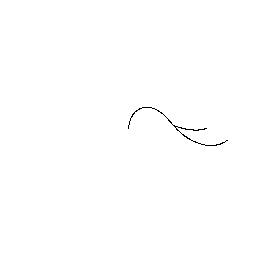
\includegraphics[width=0.6\linewidth]{example_images/CycleGAN_spline}
	\caption{Spline}
	\label{fig:Spline}
\end{figure}

\begin{figure}
	\centering
	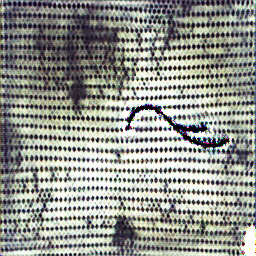
\includegraphics[width=0.6\linewidth]{example_images/CycleGAN_fakeimage}
	\caption{fakeimage}
	\label{fig:fakeimage}
\end{figure}
After training with the 2000 virtual images created by CycleGAN network, the prediction results are in \autoref{Pretraining Results}.
\begin{figure}
	\centering
	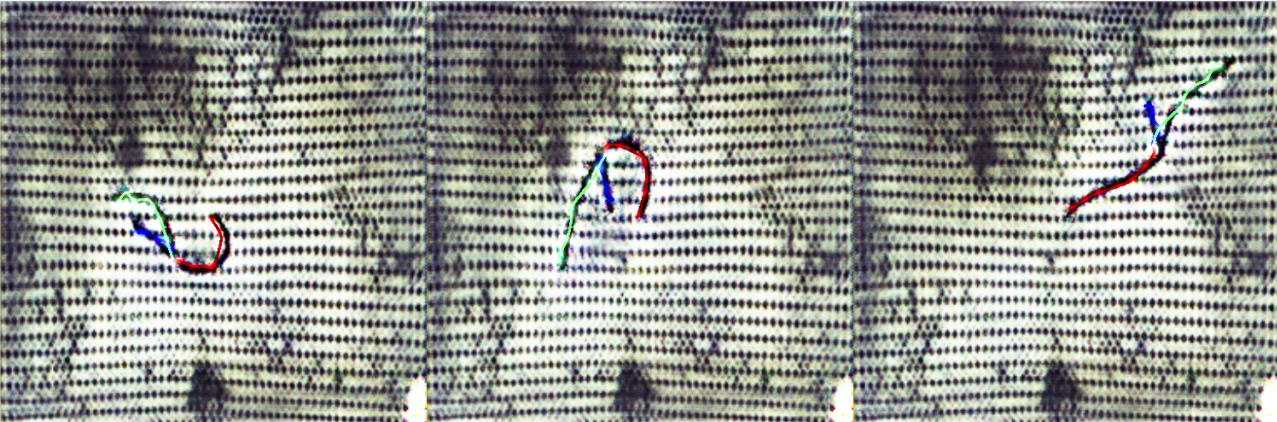
\includegraphics[width=0.6\linewidth]{example_images/PretrainingResultCycleGAN}
	\caption{Validation Results of pretraining}
	\label{Pretraining Results}
\end{figure}
And the model is trained again with the real images by transfer learning. The validation loss is $20\%$ lower than not using pretraining. An example of validated result is 
\autoref{Validation Results using transfer learning}
\begin{figure}
	\centering
	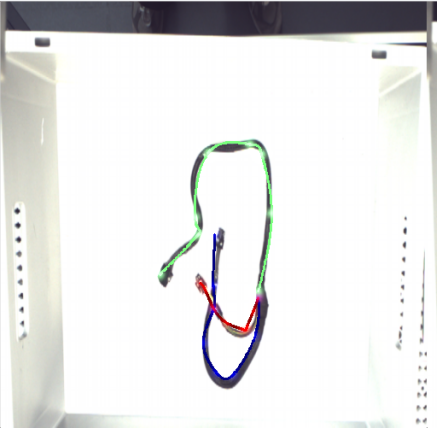
\includegraphics[width=0.6\linewidth]{example_images/usePretraining_NoTransformer}
	\caption{Validation Results of model using transfer learning}
	\label{Validation Results using transfer learning}
\end{figure}


\subsubsection{Expand Dataset by operations on segments} 
To operate on the branches of the harness, the harness first needs to be segmented. Here the images are firstly segmented to individual segments by using
Label-Studio, see \autoref{fig:Wire Segmentation}.\\
\begin{figure}
	\centering
	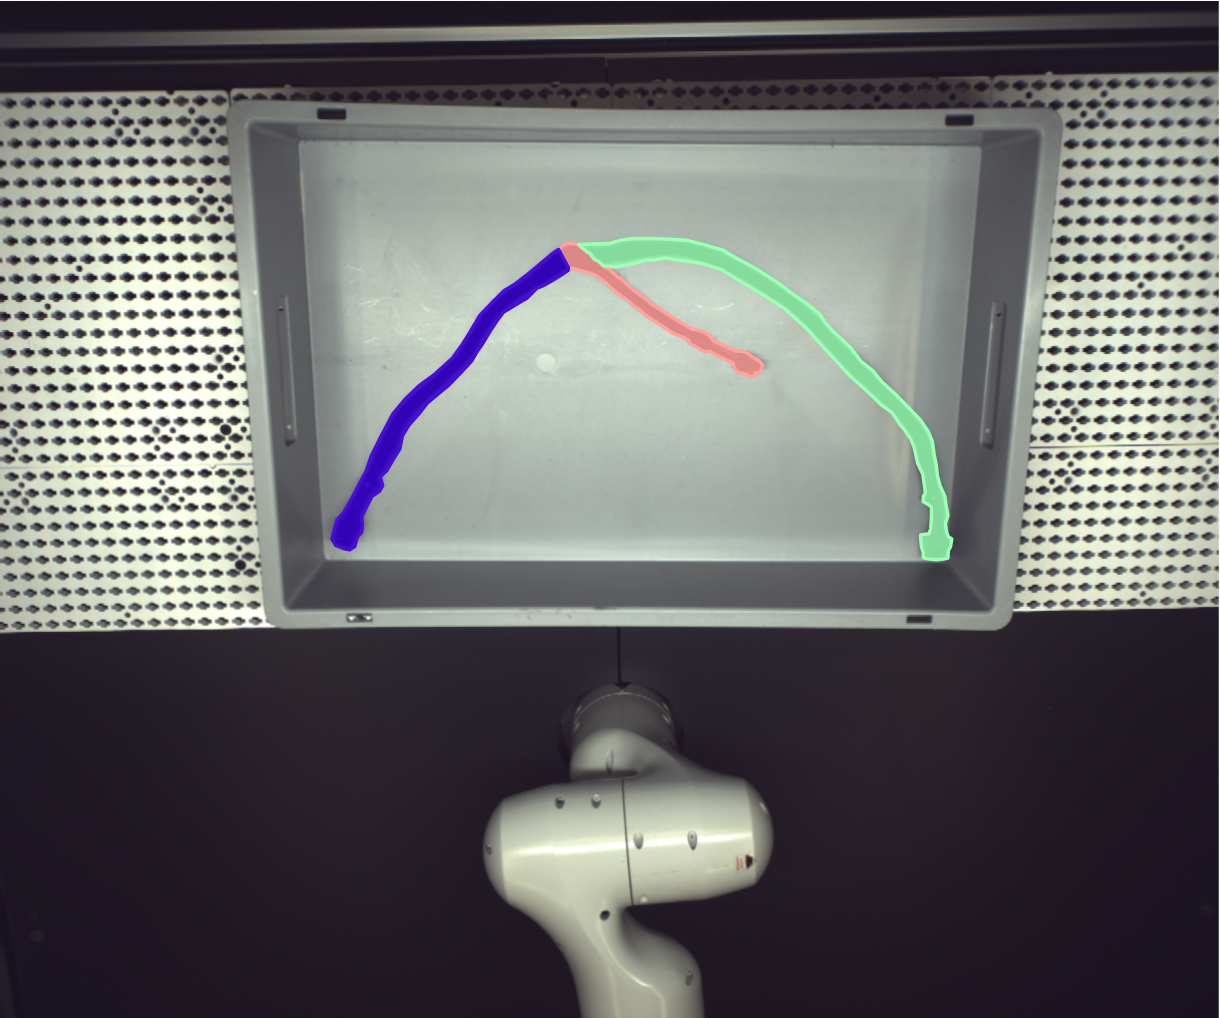
\includegraphics[width=0.6\linewidth]{example_images/img_0_segment}
	\caption{Wire Segmentation}
	\label{fig:Wire Segmentation}
\end{figure}
A rotation matrix is defined as \autoref{eq:rotation matrix}:
\begin{align}
	\begin{bmatrix}
		cos(\theta)&  -sin(\theta )&x \\
		sin(\theta )&  cos(\theta )&y  \\
		0&  0&1
	  \end{bmatrix} \label{eq:rotation matrix}
\end{align}
An all-zeros mask will be created firstly that has the same size as the image of wire harnesses. The values on mask, where corresponds to the coordinate position of
annotated points of segmentation, are then equal to one. The corresponding image region $\mho$ of the wire harness will be segmented as a polygonal region based on the mask.
Build the rotation matrix relative to the desired position and then calculate its corresponding new coordinates by using \autoref{eq:new region}. 
Paste the previously segmented polygonal area onto the empty background. The new generated virtual image is \autoref{fig:fake image}.
\begin{align}
	\mho ^{\star } = \mho \cdot \begin{bmatrix}
		cos(\theta)&  -sin(\theta )&x \\
		sin(\theta )&  cos(\theta )&y  \\
		0&  0&1
	  \end{bmatrix} \label{eq:new region}
\end{align}

\begin{figure}
	\centering
	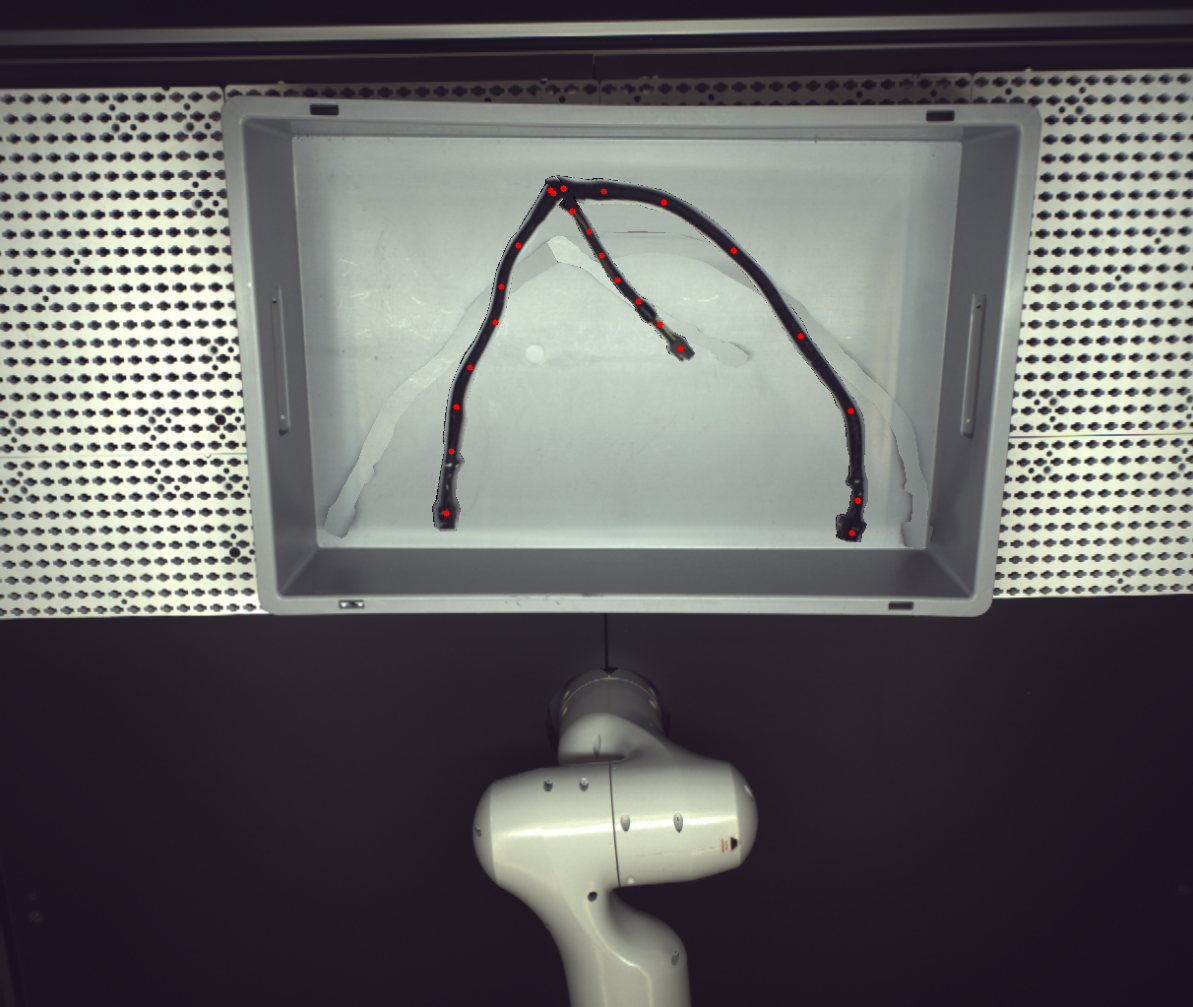
\includegraphics[width=0.6\linewidth]{example_images/img_0_segment_fakeImages}
	\caption{fake image}
	\label{fig:fake image}
\end{figure}
The corresponding annotation $\Theta $ could also be calculated with the rotation matrix as \autoref{eq:new anno}:
\begin{align}
	\Theta ^{\star } = \Theta \cdot \begin{bmatrix}
		cos(\theta)&  -sin(\theta )&x \\
		sin(\theta )&  cos(\theta )&y  \\
		0&  0&1
	  \end{bmatrix} \label{eq:new anno}
\end{align}
